\documentclass[answers]{exam} % Clase para exámenes con respuestas
\usepackage[english,spanish]{babel} % Soporte para inglés y español
\usepackage[autostyle]{csquotes} % Manejo de citas
\usepackage{amsmath, amssymb} % Paquetes para matemáticas avanzadas
\usepackage{graphicx} % Inclusión de gráficos
\usepackage{enumitem} % Personalización de listas enumeradas
\usepackage[letterpaper,top=2cm,bottom=2cm,left=1.5cm,right=1.5cm]{geometry} % Márgenes ajustados para mayor ancho de contenido
\usepackage[colorlinks=true, allcolors=blue]{hyperref} % Enlaces con color
\usepackage{wrapfig}
\usepackage{graphicx}

\usepackage{array}   % for adjusting row height
\renewcommand{\arraystretch}{1.5} % adjust the vertical spacing between rows
\usepackage{multicol}
\usepackage{tikz}


\renewcommand{\solutiontitle}{\noindent\textbf{Respuesta:}\par\noindent} % Personalización del título de respuestas
\renewcommand{\familydefault}{\sfdefault}

% Configuración de encabezado y pie de página
\pagestyle{headandfoot}
\firstpageheader{Universidad de Bolívar}{}{15 de Octubre del 2024} 
\runningheader{Universidad de Bolívar}{}{Física}
\firstpagefooter{}{\thepage}{}
\runningfooter{}{\thepage}{}

\begin{document}

\begin{center}
	\large\textbf{Trabajo Autónomo 1.6 - Fundamentos de Física para Ingeniería}\\[1em]
	\large Segundo Ciclo \enquote*{A} - Ingeniería de Software\\[1em]
\end{center}

\vspace{0.5cm}
\noindent
\large\textbf{Tema:} Potencial eléctrico \\
\large\textbf{Estudiante:} Ariel Alejandro Calderón 
\vspace{0.5cm}

\begin{questions}

	% Question 1
	\question \large\textbf{¿A qué distancia en el vacío de una carga de 100 C el potencial es de 2V?.}
	\vspace{0.5cm}

	El potencial eléctrico \( V \) debido a una carga puntual \( q \) en el vacío a una distancia \( r \) está dado por la fórmula:

	\[
		V = \frac{1}{4 \pi \varepsilon_0} \frac{q}{r} \implies r = \frac{1}{4 \pi \varepsilon_0} \frac{q}{V}
	\]

	Donde:
	\begin{itemize}
		\item \( V \) es el potencial eléctrico (en voltios),
		\item \( q \) es la magnitud de la carga (en culombios),
		\item \( \varepsilon_0 \) es la constante de permitividad eléctrica del vacío (\( \varepsilon_0 \approx 8.854 \times 10^{-12} \, \text{F/m} \)),
		\item \( r \) es la distancia entre la carga y el punto donde se mide el potencial (en metros).
	\end{itemize}

	\[
		r = \frac{1}{4 \pi (8.854 \times 10^{-12})} \frac{100}{2} \implies r \approx 4.493 \times 10^9 \, \text{m}
	\]


	Por lo tanto, la distancia es aproximadamente \( 4.49 \times 10^9 \, \text{m} \).

	\vspace{0.5cm}

	% Question 2
	\question \large\textbf{Dos cargas de 0.02 C y 0.03 C separadas 10 cm en el vacío. Calcular el potencial (a)
		en el punto medio de la recta que las une, (b) en un punto a 2 cm de la primera y
		entre ellas, y (c) en un punto a 4 cm de la primera y fuera de ellas.}

	\vspace{0.5cm}

	\begin{enumerate}[label=\alph*)]
		\item \textbf{En el punto medio de la recta que une a las dos cargas:}

		      En el punto medio, las distancias de ambas cargas al punto son iguales, es decir, \( r_1 = r_2 = \frac{d}{2} = 0.05 \, \text{m} \). El potencial total es la suma de los potenciales debidos a cada carga:

		      \[
			      V = \frac{1}{4 \pi \varepsilon_0} \left( \frac{q_1}{r_1} + \frac{q_2}{r_2} \right)
		      \]

		      Sustituyendo los valores:

		      \[
			      V = \frac{1}{4 \pi (8.854 \times 10^{-12})} \left( \frac{0.02}{0.05} + \frac{0.03}{0.05} \right)
		      \]

		      Realizando los cálculos:

		      \[
			      V \approx 1.0806 \times 10^{11} \, \text{V}
		      \]

		\item \textbf{En un punto a 2 cm de la primera carga y entre ellas:}

		      En este caso, la distancia de la primera carga es \( r_1 = 0.02 \, \text{m} \), y la distancia de la segunda carga es \( r_2 = 0.08 \, \text{m} \). El potencial total es:

		      \[
			      V = \frac{1}{4 \pi \varepsilon_0} \left( \frac{q_1}{r_1} + \frac{q_2}{r_2} \right)
		      \]

		      Sustituyendo los valores:

		      \[
			      V = \frac{1}{4 \pi (8.854 \times 10^{-12})} \left( \frac{0.02}{0.02} + \frac{0.03}{0.08} \right)
		      \]

		      Realizando los cálculos:

		      \[
			      V \approx 1.125 \times 10^{11} \, \text{V}
		      \]

		\item \textbf{En un punto a 4 cm de la primera carga y fuera de ellas:}

		      Aquí, la distancia de la primera carga es \( r_1 = 0.04 \, \text{m} \), y la distancia de la segunda carga es \( r_2 = 0.06 \, \text{m} \). El potencial total es:

		      \[
			      V = \frac{1}{4 \pi \varepsilon_0} \left( \frac{q_1}{r_1} + \frac{q_2}{r_2} \right)
		      \]

		      Sustituyendo los valores:

		      \[
			      V = \frac{1}{4 \pi (8.854 \times 10^{-12})} \left( \frac{0.02}{0.04} + \frac{0.03}{0.06} \right)
		      \]

		      Realizando los cálculos:

		      \[
			      V \approx 8.9876 \times 10^{10} \, \text{V}
		      \]
	\end{enumerate}

	\begin{center}
		\begin{tikzpicture}
			% Definir las posiciones de las cargas y los puntos de interés
			\coordinate (q1) at (0, 0);       % Posición de q1
			\coordinate (q2) at (10, 0);      % Posición de q2
			\coordinate (mid) at (5, 0);      % Punto medio
			\coordinate (p1) at (2, 0);       % Punto a 2 cm de q1
			\coordinate (p2) at (-4, 0);      % Punto a 4 cm de q1 (afuera)

			% Dibujar las cargas
			\filldraw[red] (q1) circle (0.15) node[above] {$q_1 = 0.02 \, \text{C}$};
			\filldraw[blue] (q2) circle (0.15) node[above] {$q_2 = 0.03 \, \text{C}$};

			% Dibujar los puntos de interés
			\draw[black, fill=black] (mid) circle (0.08) node[below] {Punto medio};
			\draw[black, fill=black] (p1) circle (0.08) node[below] {2 cm de $q_1$};
			\draw[black, fill=black] (p2) circle (0.08) node[below] {4 cm de $q_1$};

			% Dibujar la distancia entre las cargas
			\draw [thick] (p2) -- (q2) ;

		\end{tikzpicture}
	\end{center}

	\vspace{0.5cm}

	% Question 3
	\question \large\textbf{¿Cuál es la diferencia de potencial entre dos puntos si para transportar una carga de 12.5 C el campo realiza un trabajo de 6.25 J?}

	La relación entre el trabajo \(W\), la carga \(q\), y la diferencia de potencial \(\Delta V\) está dada por la ecuación:

	\[
		W = q \cdot \Delta V
	\]

	De esta expresión, despejamos la diferencia de potencial:

	\[
		\Delta V = \frac{W}{q}
	\]

	Sustituyendo los valores dados:

	\[
		\Delta V = \frac{6.25 \, \text{J}}{12.5 \, \text{C}} = 0.5 \, \text{V}
	\]

	Por lo tanto, la diferencia de potencial entre los dos puntos es de \(0.5 \, \text{V}\).

	\begin{center}
		\begin{tikzpicture}
			% Nodos
			\node at (-2,0) [circle,draw,fill=blue!20] (A) {A};
			\node at (2,0) [circle,draw,fill=red!20] (B) {B};

			% Flecha que representa el campo eléctrico
			\draw[thick] (A) -- (B) node[midway, above] {$\vec{E}$};

			% Carga
			\node at (0,-0.5) [below] {Carga $q = 12.5 \, \text{C}$};

			% Trabajo realizado
			\node at (0, 1.5) {Trabajo $W = 6.25 \, \text{J}$};

			% Diferencia de potencial
			\node at (0,-1.5) {$\Delta V = 0.5 \, \text{V}$};
		\end{tikzpicture}
	\end{center}

	\vspace{0.5cm}
	% Question 4
	\question \large\textbf{A) Encontrar la ecuación de la superficie equipotencial generada por una carga puntual de 1 C en agua $\varepsilon_r = 80$ , B) ¿Cuál es el radio de la esfera equipotencial si el valor del potencial en cualquier punto de la esfera es de 100 V?}

	A) La ecuación del potencial eléctrico $V$ generado por una carga puntual $q$ en un medio con permitividad relativa $\varepsilon_r$ es:

	\[
		V(r) = \frac{1}{4\pi \varepsilon_0 \varepsilon_r} \cdot \frac{q}{r}
	\]

	Donde $q = 1 \, \text{C}$, $\varepsilon_r = 80$, y $\varepsilon_0 = 8.85 \times 10^{-12} \, \text{F/m}$. Por lo tanto, la expresión para el potencial en función de la distancia $r$ es:

	\[
		V(r) = \frac{1}{4\pi (8.85 \times 10^{-12})(80)} \cdot \frac{1}{r}
	\]

	B) Para encontrar el radio $r$ de la esfera igualamos la ecuación del potencial a 100 V:

	\[
		100 = \frac{1}{4\pi (8.85 \times 10^{-12})(80)} \cdot \frac{1}{r}
	\]

	Despejando $r$:

	\[
		r = \frac{1}{4\pi (8.85 \times 10^{-12})(80)} \cdot \frac{1}{100} \approx 0.113 \, \text{m}
	\]

	Por lo tanto, el radio de la esfera equipotencial es aproximadamente $r = 0.113 \, \text{m}$.

	\newpage

	\vspace{0.5cm}
	% Question 5
	\question \large\textbf{Dibuje la gráfica $V = f(r)$ que genera una partícula cargada con 1 C en el vacío.}

	\begin{figure}[h!]
		\centering
		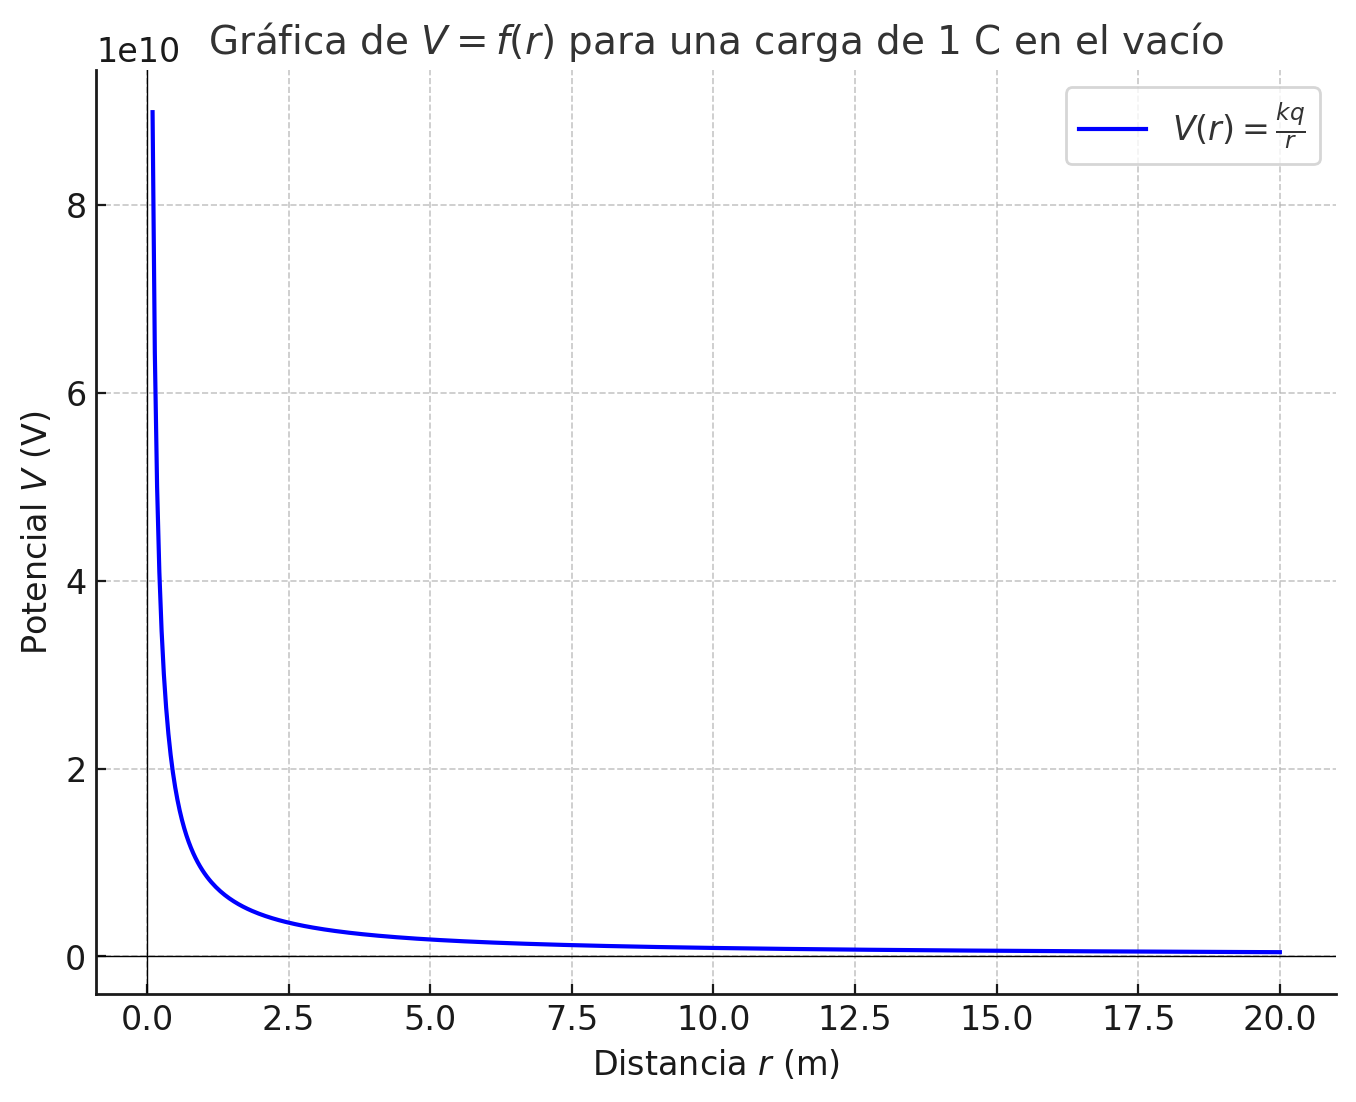
\includegraphics[width=0.63\textwidth]{./public/g1.png}
	\end{figure}

	\vspace{0.5cm}

	% Question 6
	\question \large\textbf{Calcular el trabajo necesario para tener cargas de 5 $\mu$C en los vértices de un hexágono regular de lado $a$. Recalcular el trabajo para cuando $a = 0.25$ m.}

	Consideremos un hexágono regular con 6 vértices. Colocamos una carga \( q = 5 \, \mu\text{C} = 5 \times 10^{-6} \, \text{C} \) en cada vértice. El trabajo necesario para ensamblar el sistema es igual a la energía potencial eléctrica total del sistema.

	La energía potencial entre dos cargas puntuales \( q_1 \) y \( q_2 \), separadas por una distancia \( r \), está dada por:

	\[
		U = \frac{1}{4 \pi \varepsilon_0} \frac{q_1 q_2}{r}
	\]

	En un hexágono regular, las distancias entre las cargas pueden ser:
	\begin{itemize}
		\item \( r = a \), la distancia entre vértices adyacentes,
		\item \( r = \sqrt{3}a \), la distancia entre vértices separados por un vértice intermedio,
		\item \( r = 2a \), la distancia entre vértices opuestos.
	\end{itemize}


	El número total de pares de interacciones entre las 6 cargas es \( \binom{6}{2} = 15 \), y los pares correspondientes a cada distancia son:
	\begin{itemize}
		\item 6 pares a distancia \( a \),
		\item 6 pares a distancia \( \sqrt{3}a \),
		\item 3 pares a distancia \( 2a \).
	\end{itemize}


	Por lo tanto, la energía potencial total del sistema es:

	\[
		U_{\text{total}} = \frac{1}{4 \pi \varepsilon_0} \left[ 6 \frac{q^2}{a} + 6 \frac{q^2}{\sqrt{3}a} + 3 \frac{q^2}{2a} \right]
	\]

	Sustituyendo \( q = 5 \times 10^{-6} \, \text{C} \) y \( \varepsilon_0 = 8.854 \times 10^{-12} \, \text{C}^2/\text{N}\cdot\text{m}^2 \):

	\[
		U_{\text{total}} = \frac{1}{4 \pi (8.854 \times 10^{-12})} \left[ 6 \frac{(5 \times 10^{-6})^2}{a} + 6 \frac{(5 \times 10^{-6})^2}{\sqrt{3}a} + 3 \frac{(5 \times 10^{-6})^2}{2a} \right]
	\]

	Simplificando:

	\[
		U_{\text{total}} = \frac{9 \times 10^9}{a} \left[ 6 (25 \times 10^{-12}) + 6 \frac{25 \times 10^{-12}}{\sqrt{3}} + 3 \frac{25 \times 10^{-12}}{2} \right]
	\]

	Calculamos la energía total para cuando \( a = 0.25 \, \text{m} \):

	\[
		U_{\text{total}} = \frac{9 \times 10^9}{0.25} \left[ 6 (25 \times 10^{-12}) + 6 \frac{25 \times 10^{-12}}{\sqrt{3}} + 3 \frac{25 \times 10^{-12}}{2} \right] = 1.008 \, \text{J}
	\]

	Por lo tanto, el trabajo necesario para ensamblar las cargas en los vértices del hexágono es de \( 1.008 \, \text{J} \) cuando \( a = 0.25 \, \text{m} \).

	\begin{figure}[h!]
		\centering
		\begin{tikzpicture}[scale=3]
		
		% Dibujar el hexágono
		\foreach \x in {1,...,6} {
			\draw[thick] ({60*(\x-1)}:1) -- ({60*(\x)}:1);
		}
		
		% Etiquetar los vértices con las cargas
		\foreach \x in {1,...,6} {
			\node[draw, circle, inner sep=1pt, fill=red] at ({60*(\x-1)}:1) {};
			\node at ({60*(\x-1)}:1.15) {$5 \, \mu C$};
		}
		
		% Etiquetar las longitudes de los lados
		\foreach \x in {1,...,6} {
			\draw[<-] ({60*(\x-1)}:1.05) arc[start angle=60*(\x-1), end angle=60*(\x), radius=1.05];
		}
		\node at (0.7,0) {$a$};
		
		% Dibujar el centro
		\draw[fill] (0,0) circle (0.02);
		\node at (0,0.1) {Centro};
		
		\end{tikzpicture}
		\caption{Distribución de cargas en los vértices de un hexágono regular de lado $a$.}
		\end{figure}

	\vspace{0.5cm}


\end{questions}

\end{document}